%% LaTeX Beamer presentation template (requires beamer package)
%% see http://bitbucket.org/rivanvx/beamer/wiki/Home
%% idea contributed by H. Turgut Uyar
%% template based on a template by Till Tantau
%% this template is still evolving - it might differ in future releases!

\documentclass{beamer}

\mode<presentation>
{
\usetheme{Warsaw}

\setbeamercovered{transparent}
}

\usepackage[english]{babel}
\usepackage[latin1]{inputenc}

% font definitions, try \usepackage{ae} instead of the following
% three lines if you don't like this look
\usepackage{mathptmx}
\usepackage[scaled=.90]{helvet}
\usepackage{courier}
\usepackage{xcolor}


\usepackage[T1]{fontenc}


\title[Predictive Active Steering Control for Autonomous Vehicle
Systems]{Example for an Model Predictive Controller
\\
for an active steering coltrol  \\
of an automomous vehicle}

%\subtitle{}

% - Use the \inst{?} command only if the authors have different
%   affiliation.
\author{Dominique Laurencelle\inst{1} \and Stefan Glaser\inst{2}}
%\author{\inst{1}}

% - Use the \inst command only if there are several affiliations.
% - Keep it simple, no one is interested in your street address.
\institute[Universities of]
{
\inst{1}%
M.Sc. ESE\\
Albert Ludwigs University, Freiburg
\and
\inst{2}%
M.Sc. Informatics\\
Albert Ludwigs University, Freiburg}

\date{19.7.2016 / OMPC Seminar}


% This is only inserted into the PDF information catalog. Can be left
% out.
\subject{Talks}



% If you have a file called "university-logo-filename.xxx", where xxx
% is a graphic format that can be processed by latex or pdflatex,
% resp., then you can add a logo as follows:

% \pgfdeclareimage[height=0.5cm]{university-logo}{university-logo-filename}
% \logo{\pgfuseimage{university-logo}}



% Delete this, if you do not want the table of contents to pop up at
% the beginning of each subsection:
\AtBeginSubsection[]
{
\begin{frame}<beamer>
\frametitle{Outline}
\tableofcontents[currentsection,currentsubsection]
\end{frame}
}

% If you wish to uncover everything in a step-wise fashion, uncomment
% the following command:

%\beamerdefaultoverlayspecification{<+->}

\begin{document}

\begin{frame}
\titlepage
\end{frame}

% \begin{frame}
% \frametitle{Outline}
% \tableofcontents
% % You might wish to add the option [pausesections]
% \end{frame}


%============================================================
%=========================== LIPM ===========================
%============================================================
\section*{Section name}

\subsection*{Subsection1 name}
\subsection*{Subsection2 name}

\begin{frame}
\frametitle{My Frametitle}
%\framesubtitle{Subtitles are optional}

\begin{columns}[t,onlytextwidth]
\column{.5\textwidth}
Some stuff here

\column{.5\textwidth}
and some more here

\end{columns}

\end{frame}






\begin{frame}
\frametitle{My Frametitle2}

My second frame

\end{frame}





\begin{frame}
\frametitle{System Overview}

\begin{figure} [h]
\begin{center}
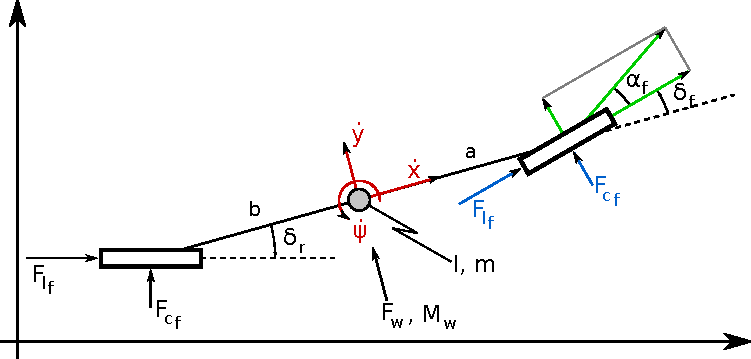
\includegraphics[scale=0.8]{images/dynamics_overview.pdf}
\label{fig:pendel}
\end{center}
\end{figure}
\[F_l : \text{Longitudial (tractive) force [N]} \qquad F_c : \text{Lateral
(cornering) force [N]]}\] \[v_l : \text{Longitudial (tractive) velocity [m/s]]}
\qquad v_l : \text{Lateral (cornering) velocity}\] \[\dot{x}, \dot{y} :
\text{local velocities [m/s]} \qquad \dot{\psi} :
\text{angular velocity [1/s]}\]

\end{frame}





\begin{frame}
\frametitle{System overview}

% \begin{align*}
% v_{y_f} &= \dot{y} + a \dot{\psi}, & v_{y_r} &= \dot{y} - b \dot{\psi} \\
% v_{x_f} &= \dot{x}, & v_{x_r} &= \dot{x}
% \end{align*}
\begin{block}{System state and input}
\[\xi = [\dot{x}, \dot{y}, \psi, \dot{\psi}, X, Y] \qquad \qquad u = \delta_f\]
\end{block}

\begin{columns}[t,onlytextwidth]
\column{.45\textwidth}
\begin{block}{Vehicle dynamics}
\begin{align*}
\ddot{x} &= \dot{y} \dot{\psi} + \frac{2}{m} (F_{x_f} + F_{x_r}) \\
\ddot{y} &= - \dot{x} \dot{\psi} + \frac{2}{m} (F_{y_f} + F_{y_r}) \\
\ddot{\psi} &= \frac{2}{I} (a F_{y_f} - b F_{y_r}) \\
\dot{X} &= \dot{x} \ cos \psi - \dot{y} \ sin \psi \\
\dot{Y} &= \dot{x} \ sin \psi + \dot{y} \ cos \psi
\end{align*}
\end{block}

\column{.45\textwidth}
\begin{block}{Forces (front and rear wheels)}
\begin{align*}
F_x &= F_l \ cos \delta - F_c \ sin \delta \\
F_y &= F_l \ sin \delta + F_c \ cos \delta
\end{align*}
Pacejka tire model:
\begin{align*}
F_l &= f_l(\alpha, s, F_z) \\
F_c &= f_c(\alpha, s, F_z)
\end{align*}
\end{block}

\end{columns}

\end{frame}





\begin{frame}
\frametitle{Trajectory generation}

\begin{align*}
Y_{ref}(X) &= 2.025 \ (1 + tanh(z_1)) - 2.85 \ (1 + tanh(z_2)) \\
\psi_{ref}(X) &= tan^{-1} \left( 0.1944 \ \left(\frac{1}{cosh(z_1)}\right)^2 - 0.311 \ \left(\frac{1}{cosh(z_2)}\right)^2 \right)
\end{align*}
\[\quad \text{with} \quad z_1 = \frac{2.4}{25}(X - 27.19) - 1.2 \qquad z_2 = \frac{2.4}{21.95}(X - 56.46) \]


\begin{columns}[t,onlytextwidth]
\column{.45\textwidth}
Y-reference image

\column{.45\textwidth}
Psi-reference image

\end{columns}

\end{frame}






\begin{frame}
\frametitle{Optimization problem}

\begin{block}{Objective function}


\begin{align*}
J(\xi_t, \Delta U_t) = &\sum_{i=1}^{H_p} \left( ||\xi_i(6) - Y_{ref}(\xi_i(5)) ||_{75}^2 + ||\xi_i(3) - \psi_{ref}(\xi_i(5)) ||_{500}^2 \right) \\
&+ \sum_{i=0}^{H_c-1} || \Delta u_i ||_{150}^2
\end{align*}
\[\text{with} \quad H_p : \text{prediction horizon} \qquad H_c : \text{control
horizon}\]


\end{block}

\end{frame}







\begin{frame}
\frametitle{NLP problem formulation}

\begin{align*}
\min_{\Delta U \in \mathbb{R}^{H_p}} \quad &J(\xi_t, \Delta U_t) \\
s.t. \qquad &\xi_{k+1} = f(\xi_k, u_k) \\
&\delta_{min} \leq u_k \leq \delta_{max} \\
&\Delta \delta_{min} \leq \Delta u_k \leq \Delta \delta_{max} \\
&u_k = u_{k-1} + \Delta u_k \\
&\Delta u_k = 0, \qquad \qquad k = H_c, . . . , H_p \\
&\xi_0 = \xi_{init} \\
& u_{-1} = u_{init}
\end{align*}

\end{frame}







\begin{frame}
\frametitle{LTV problem formulation}

\begin{align*}
\min_{\Delta U \in \mathbb{R}^{H_p}} \quad &J(\xi_t, \Delta U_t) + \rho \epsilon \\
s.t. \qquad &\xi_{k+1} = A_t \xi_k + B_t u_k \\
&\alpha_{k+1} = C_t \xi_k + D_t u_k \\
&\delta_{min} \leq u_k \leq \delta_{max} \\ 
&\Delta \delta_{min} \leq \Delta u_k \leq \Delta \delta_{max} \\
&\alpha_{min} - \epsilon \leq \alpha_k \leq \alpha_{max} + \epsilon \\
&u_k = u_{k-1} + \Delta u_k \\
&\Delta u_k = 0, \qquad \qquad k = H_c, . . . , H_p \\
&\epsilon \geq 0 \\
&\xi_0 = \xi_{init} \\
& u_{-1} = u_{init}
\end{align*}

\end{frame}







\begin{frame}
\frametitle{System Overview}
Results. . .

\end{frame}


% \begin{frame}
% \frametitle<presentation>{Summary}
% 
% \begin{itemize}
%   \item The \alert{first main message} of your talk in one or two lines.
% \end{itemize}
% 
% % The following outlook is optional.
% \vskip0pt plus.5fill
% \begin{itemize}
%   \item Outlook
%   \begin{itemize}
%     \item Something you haven't solved.
%     \item Something else you haven't solved.
%   \end{itemize}
% \end{itemize}
% \end{frame}

\end{document}
